\documentclass[isoft]{ssltexposter}

\usepackage{lipsum}
\usepackage{natbib}
\usepackage{booktabs}
\usepackage{subfig} 
\usepackage{amsmath} 
\usepackage{textcomp} 
\usepackage{color}
\usepackage{url}  
\usepackage[hidelinks]{hyperref}
\usepackage[utf8]{inputenc}
%\usepackage[brazil, english]{babel}
\usepackage[spanish]{babel}
\usepackage[pages=some]{background}
\usepackage{enumitem}
\usepackage{fontawesome}
\usepackage{cancel}
\usepackage{steinmetz}


\usepackage{colortbl}

\definecolor{MediumBlue}{rgb}{0.01176, 0.31372, 0.43529}

%%%%%%%%%%%%%%%%%%%%%%%%%%%%%%%%%%%%%%%%%
%%               Configs               %%
%%%%%%%%%%%%%%%%%%%%%%%%%%%%%%%%%%%%%%%%%

% Choose one of the section color {ufglhblue | ufgdkblue | dkblue | black | gold}
\setsectioncolor{black}


% Define width of the rule or hide it by setting 0pt or commenting the command 
\setcolumnseprule{0pt}

% Inform the paths to the logo files or leave empty one or both parameters. 
% There are three options [ T | M | B ] to positioning them.
\setlogos[T]{}{}

% Choose one of the background options {1 | 2 | 3}. 
% Actually, one can select any graphic file in backgrounds directory. 
%\setbackground{1c}

% Resize the title to keep it in two lines // {font size}{line height}
\settitlesize{64pt}{68pt}

% Resize the font of the content. Default {32pt}{38pt} // {font size}{line height}
\setcontentfontesize{32pt}{40pt}

% Resize the font of the emails. Default {26pt}{32pt} // {font size}{line height}
\setemailfontesize{42pt}{40pt}

% General info
\title{\uppercase{Análisis de sistemas \\ no lineales: Diodos} \\ \small{OTP-ONDY-010-Ver.A-Rev.02}} 

\author{Departamento de ingeniería} 

% \department{Laboratório de Sinais e Sistemas\\Universidade Federal do ABC (UFABC)}


%\email{Onduladores de Chile S.A }

% \class{I Workshop do Laboratório de Sinais e Sistemas (WLSS)}

% \year{2019}

\conference{}

%%%%%%%%%%%%%%%%%%%%%%%%%%%%%%%%%%%%%%%%%
%%           End configs               %%
%%%%%%%%%%%%%%%%%%%%%%%%%%%%%%%%%%%%%%%%%


\begin{document}
    \begin{poster}
    %%%%%%%%%%%%%%%%%%%%%%%%%%%%%%%%%%%%%%%%%
    %%             Begin poster            %%
    %%%%%%%%%%%%%%%%%%%%%%%%%%%%%%%%%%%%%%%%%

\setbackground{1}   
\cfoot{\thepage} 
\section{Introducción}
El diodo es un elemento que tiene una predominancia alta en la electrónica moderna. Se trata de un componente semiconductor que actúa como una válvula eléctrica unidireccional, permitiendo que la corriente fluya en una dirección mientras la bloquea eficazmente en la opuesta. Esta característica única ha convertido al diodo en una piedra angular de la tecnología, desempeñando un papel crucial en una amplia gama de dispositivos y circuitos electrónicos. Desde su uso en rectificadores para convertir la corriente alterna en continua, hasta su presencia en la tecnología de iluminación LED y en la protección de circuitos contra polaridad inversa, el diodo sigue siendo un componente esencial en la electrónica contemporánea que continúa impulsando la innovación tecnológica.

La confección de este informe se llevó a cabo utilizando como guía el libro \cite{teoria_circuitos_boylestad}, el cual está orientado al análisis de circuitos no lineales. 

\section{Diodos}

\subsection{Definición y funcionamiento.}
Un diodo es un componente electrónico de dos terminales que permite el flujo de corriente eléctrica en una dirección mientras bloquea su flujo en la dirección opuesta. Está construido con materiales semiconductores y tiene una estructura de unión PN, donde una región tipo P se une con una región tipo N. Esta unión PN es fundamental para su funcionamiento.

Los materiales tipo N y P se crean mediante la adición controlada de impurezas a una matriz de silicio, a menudo en una proporción de aproximadamente una parte en diez millones. En el caso de un material tipo N, se incorporan impurezas que posean cinco electrones en su capa de valencia, como antimonio, arsénico o fósforo. Esta configuración permite que exista un electrón adicional en la capa de valencia, que no forma pares con otros electrones y, por lo tanto, está relativamente libre para moverse dentro del material. Por otro lado, el material tipo P se dopa con impurezas que tienen tres electrones en su capa de valencia, como boro, galio o indio. Esta mezcla resulta en un déficit de electrones para completar la estructura covalente de la banda, formada por estos dos materiales.


\begin{figure}
    \centering
    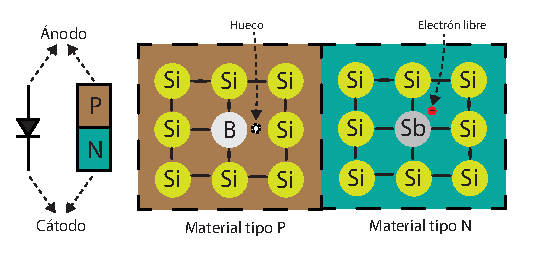
\includegraphics[width=0.4\textwidth]{imagenes/diodo.eps}
    \caption{Modelo del diodo y su composición interna.}
    \label{fig:diodo}
\end{figure}



Cuando se aplica una tensión positiva entre ánodo y cátodo, la unión PN se polariza en forma directa. En esta condición, el diodo permite que la corriente fluya fácilmente, ya que los electrones pueden moverse de la región tipo N a la región tipo P, creando una baja resistencia. Por otro lado, se aplica una tensión negativa entre ánodo y cátodo, la unión PN se polariza en forma inversa. En esta configuración, el diodo actúa como un circuito abierto, bloqueando  el flujo de corriente. Es importante destacar que, en este análisis, la potencia disipada por un diodo ideal es nula. Esto se debe a que cuando el diodo conduce corriente, el voltaje a través de él es igual a cero, y cuando bloquea el voltaje inverso, su corriente también es igual a cero. Por lo tanto, se tiene que:

\begin{equation*}
    Pot_d= Vi=\underbrace{0\cdot i}_{conduccion}= \underbrace{V\cdot 0}_{bloqueo} = 0 \textup{ [W]} 
\end{equation*}


En un diodo real, la corriente comienza a fluir cuando el voltaje $V_o$ aplicado desde el ánodo al cátodo alcanza o supera los $0.7$  voltios, y la magnitud de esta corriente está limitada por un valor máximo que el diodo puede transportar sin sufrir daños. Además, en la región de polarización inversa, se observa una corriente inversa mínima, también conocida como corriente de fuga, que fluye a través del diodo, pero es extremadamente pequeña. A diferencia del modelo real, este disipa una cantidad pequeña de energía que termina por elevar su temperatura interna. 

También, es importante destacar la zona de avalancha, una región específica de funcionamiento de un diodo. En esta zona, se experimenta un aumento repentino y no controlado de la corriente inversa cuando se aplica un voltaje inverso que supera el voltaje de ruptura. Este incremento súbito se debe a que los electrones en la región de unión PN adquieren suficiente energía para liberar otros electrones mediante colisiones sucesivas. Esto genera una avalancha de electrones que aumenta de manera significativa la corriente inversa y puede dañar el diodo si no se limita adecuadamente.

La zona de avalancha es un fenómeno no deseado en la mayoría de las aplicaciones de diodos, ya que puede dañar el dispositivo y provocar un mal funcionamiento del circuito. Sin embargo, en ciertos diodos especiales llamados diodos Zener, se utiliza de manera controlada para mantener un voltaje constante en el circuito cuando se supera su voltaje de ruptura.



\begin{figure}
    \centering
    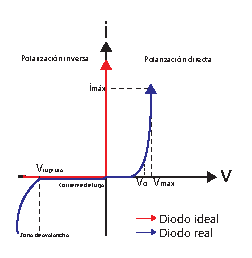
\includegraphics[width=0.25\textwidth]{imagenes/grafico_diodo.eps}
    \caption{Gráfico del modelo del diodo ideal y real.}
    \label{fig:grafico_diodo}
\end{figure}

\subsection{Otros tipos de diodos.}

\begin{itemize}
    \item \textbf{LED (Light Emitting Diode)}: Es un dispositivo semiconductor que emite luz cuando una corriente eléctrica fluye a través de él. La emisión de luz se produce debido al proceso de recombinación de electrones y huecos en la región de unión PN del diodo, liberando energía en forma de fotones.
    \item \textbf{Zener}: Es un tipo especial de diodo diseñado para operar en la región de ruptura de forma controlada. Cuando se polariza inversamente y se alcanza su tensión de ruptura, el diodo Zener mantiene un voltaje constante en sus terminales, actuando como un regulador de voltaje.
    \end{itemize}

\begin{figure}
    \centering
    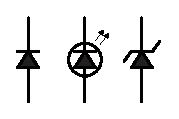
\includegraphics[width=0.1\textwidth]{imagenes/tipos_diodos.eps}
    \caption{Tipos de diodos: Diodo, LED y Zener.}
    \label{fig:tipo_diodos}
\end{figure}

\subsection{Algunas aplicaciones de los diodos.}

Los diodos tienen una amplia gama de aplicaciones en la electrónica y la industria. Algunas de las aplicaciones más comunes incluyen:

\begin{itemize}
    \item Rectificación de corriente: Se utilizan en circuitos rectificadores para convertir la corriente alterna (CA) en corriente continua (CC). Esto es esencial en la alimentación de dispositivos electrónicos.
    \item Protección contra polaridad inversa y/o sobretensiones: Los diodos se usan para proteger circuitos electrónicos de daños causados por la conexión incorrecta de la polaridad de la fuente de alimentación.
    \item  Modulación y conmutación de señales: Los diodos se emplean en aplicaciones de modulación de señales, como en la construcción de osciladores y moduladores de amplitud.
    \item Iluminación LED: Los diodos emisores de luz (LED) son un tipo especial de diodo que emite luz cuando se les aplica una corriente. Se utilizan en pantallas, indicadores luminosos y como fuentes de iluminación eficiente.
\end{itemize}
    


\newpage
\BgThispage
\section{Parámetros de rendimiento de convertidores AC-DC}

Para evaluar el desempeño de un rectificador es fundamental determinar el valor promedio y eficaces del voltaje y corriente. Estos se realizan de acuerdo con las ecuaciones \ref{valor_medio_voltaje} y \ref{valor_RMS_voltaje}. Por otro lado, la corriente se determina aplicando la Ley de Ohm en este contexto específico.

\begin{equation}
\label{valor_medio_voltaje}
    V_{x,dc}= \frac{1}{T}\int_0^T V_x(t) \mathrm{d}t \longrightarrow \textup{Valor DC de x}
\end{equation}

\begin{equation}
    \label{valor_RMS_voltaje}
    V_{x,rms}= \sqrt{\frac{1}{T} \int_0^T V_x(t)^2 \mathrm{d}t} \longrightarrow \textup{Valor RMS de x}
\end{equation}

Los parámetros de interés para medir el rendimiento se presentan a continuación:

\begin{equation}
    \eta = \frac{P_{dc}}{P_{ac}} = \frac{V_{R,dc}\cdot i_{R,dc}}{V_{f,rms}\cdot i_{f,rms}} \longrightarrow \textup{Eficiencia}
\end{equation}

\begin{equation}
    FF = \frac{V_{R,rms}}{V_{R,dc}} \longrightarrow \textup{Factor de forma}
\end{equation}

\begin{equation}
    RF= \frac{V_{ca}}{V_{dc}} = \frac{\sqrt{V_{R,rms}^2-V_{R,dc}^2}}{V_{R,dc}} \longrightarrow \textup{Factor de rizo}
\end{equation}

\begin{equation}
    FD= cos\phi = \frac{P_{act}}{S_{1}}\longrightarrow \textup{Factor de desplazamiento}
\end{equation}

\begin{equation}
    THDi=\sqrt{\left( \frac{i_{f,rms}}{i_{f-1,rms}}\right)^2-1} \longrightarrow \textup{Distorsión total armónica}
\end{equation}

\begin{equation}
    FP= \frac{P}{S}= \frac{V_{R,rms}\cdot i_{R,rms}}{V_{f,rms}\cdot i_{f,rms}}  \longrightarrow \textup{Factor de potencia}
\end{equation}
\vspace{0.2in}

El subíndice \textit{R} denota las variables asociada a la carga resistiva, mientras que el \textit{f} está ligado con la fuente. El número 1 como subíndice indica el valor de la primera armónica.
Un rectificador ideal debería presentar las siguientes características: $\eta=1$, $V_{ac}=0$, $RF=0$, $THD=0$ y $FP=1$.


\section{Rectificadores en base a diodos}
\subsection{Rectificador de media onda.}

En un circuito de media onda, se rectifica solo la mitad de un ciclo de una señal alterna.  Utiliza un solo diodo en serie con la carga. El diodo permite que la corriente fluya solo durante la mitad del ciclo de la señal de entrada, bloqueando la otra mitad.
Cuando la señal de entrada es positiva en relación con el cátodo del diodo, el diodo conduce, permitiendo que la corriente fluya a través de la carga en la dirección del flujo de la señal AC. Cuando la señal se vuelve negativa en relación con el cátodo, el diodo se polariza en inversa y bloquea el flujo de corriente.
La salida rectificada es pulsante y solo contiene la parte positiva o negativa de la señal de entrada, dependiendo de la dirección del diodo.
Este tipo de rectificación se utiliza en aplicaciones simples o donde se necesita una conversión parcial de AC a DC, pero no es eficiente ni produce una salida de CC constante.

\begin{figure}
    \centering
    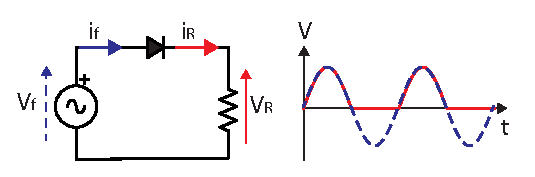
\includegraphics[width=0.4\textwidth]{imagenes/rectificador_media_onda.eps}
    \caption{Rectificador de media onda.}
    \label{fig:rectificador_media_onda}
\end{figure}



\subsection{Rectificador de onda completa}

En un circuito de onda completa, se rectifican ambas mitades de un ciclo de señal alterna.
Utiliza un puente de diodos que consta de cuatro diodos dispuestos en una configuración específica.
El puente de diodos permite que la corriente fluya en ambas direcciones a través de la carga, produciendo una salida rectificada que incluye tanto la parte positiva como la negativa de la señal de entrada.
A medida que la señal de entrada cambia de polaridad, los diodos se encienden y apagan en secuencia, garantizando que la corriente fluya en una sola dirección a través de la carga.
Este circuito es comúnmente utilizado en fuentes de alimentación de CA a CC y en la mayoría de las aplicaciones donde se necesita una rectificación completa. Proporciona una salida de CC más suave y constante que el circuito de media onda. Para mejorar el voltaje DC, se utiliza un condensador en paralelo a la carga.

\begin{figure}
    \centering
    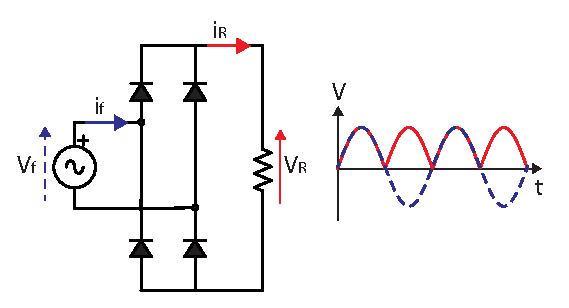
\includegraphics[width=0.30\textwidth]{imagenes/rectificador_onda_completa.eps}
    \caption{Rectificador de onda completa.}
    \label{fig:rectificador_onda_completa}
\end{figure}


\subsection{Rectificador trifásico de 6 pulsos}

El circuito de 6 pulsos es un tipo de rectificador utilizado en sistemas de alta potencia.
Esto crea seis puntos de rectificación en cada ciclo de señal de entrada (tres para cada puente de diodos), lo que proporciona una salida de CC más suave y reduce la distorsión armónica.
Los diodos se encienden y apagan en secuencia, asegurando que la corriente fluya en una sola dirección a través de la carga.
Este circuito es común en aplicaciones industriales de rectificación de alta potencia, como sistemas de alimentación de CA a CC en plantas industriales, y garantiza una salida de CC controlada y eficiente.


\begin{figure}
    \centering
    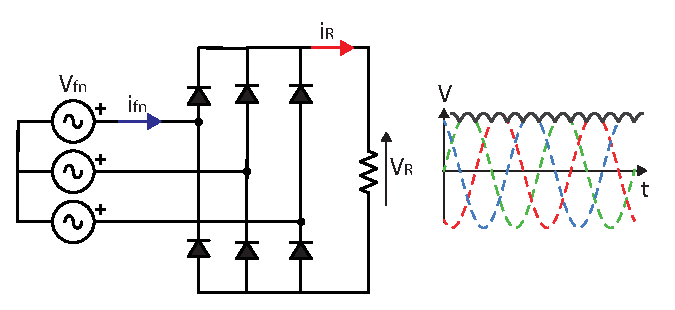
\includegraphics[width=0.30\textwidth]{imagenes/rectificador_seis_pulsos.eps}
    \caption{Rectificador trifásico de seis pulsos de cada rectificador.}
    \label{fig:rectificador_seis_pulsos}
\end{figure}

Los voltajes representados en la figura \ref{fig:rectificador_seis_pulsos} corresponden a voltajes de línea a línea, que en relación con esta configuración, son $\sqrt{3}$ veces mayores que los voltajes de fase y tienen un desfase de $30^\circ$. 

\subsection{Rendimiento de cada rectificador}

En resumen, los parámetros de cada uno de los rectificadores presentados en este informe se detallan en la tabla \ref{tab:rectificadores}. Es importante destacar que estos valores son aplicables específicamente a los rectificadores cuando la carga de salida consiste exclusivamente en una resistencia. Se observa que estos valores permanecen constantes independientemente de la magnitud de la resistencia conectada.

\vspace{0.3in}


\begin{table}
    \centering
    \begin{tabular}{|c|c|c|c|c|c|c|c|} \toprule
       \rowcolor{MediumBlue}\color{white}Tipo rectificador & \color{white} $V_{R,dc}$ & \color{white} $V_{R,RMS}$& \color{white} $\eta$& \color{white} $FF$ & \color{white} $RF$ & \color{white} $FP$\\ \midrule
         Ideal &-&-&1&1&0&1 \\
         Media onda& $\frac{V_f}{\pi}$& $\frac{V_f}{2}$& $\frac{4}{\pi^2}\sim 0.40$ &$\frac{\pi}{2}\sim 1.57$ & $1.21$ &  $0.707$ \\
         Onda completa& $\frac{2V_f}{\pi}$ & $\frac{V_f}{\sqrt{2}}$ & $\frac{8}{\pi^2}\sim 0.81$& $\frac{\pi}{2\sqrt{2}}\sim 1.11$ & $0.48$& $1$  \\  
         6 pulsos&$\frac{3\sqrt{3}V_{fn}}{\pi}$& $\sqrt{\frac{3}{2}+\frac{9\sqrt{3}}{4\pi}}V_{fn}$& $0.9983$ & $1.0008$& $0.04$& $0.956$ \\  \bottomrule
    \end{tabular}
    \caption{Parámetros de rendimiento.}
    \label{tab:rectificadores}
\end{table}


 \bibliographystyle{unsrt}
\bibliography{refs}
    
    %%%%%%%%%%%%%%%%%%%%%%%%%%%%%%%%%%%%%%%%%
    %%               End poster            %%
    %%%%%%%%%%%%%%%%%%%%%%%%%%%%%%%%%%%%%%%%%

\end{poster}
\end{document}

 
